%%%%%%%% ICML 2026 FORMATTED PAPER %%%%%%%%%%%%%%%%%

\documentclass{article}

% Recommended, but optional, packages for figures and better typesetting:
\usepackage{microtype}
\usepackage{graphicx}
\usepackage{subcaption}
\usepackage{booktabs} % for professional tables
\usepackage{amsmath}
\usepackage{amssymb}
\usepackage{mathtools}
\usepackage{amsthm}
\usepackage{hyperref}
\usepackage{algorithm}
\usepackage{algorithmic}
\usepackage{caption}

% Attempt to make hyperref and algorithmic work together better:
\newcommand{\theHalgorithm}{\arabic{algorithm}}

% Use the following line for the initial blind version submitted for review:
\usepackage{icml2026}

\usepackage{cleveref}

%%%%%%%%%%%%%%%%%%%%%%%%%%%%%%%%
% THEOREMS
%%%%%%%%%%%%%%%%%%%%%%%%%%%%%%%%
\theoremstyle{plain}
\newtheorem{theorem}{Theorem}[section]
\newtheorem{proposition}[theorem]{Proposition}
\newtheorem{lemma}[theorem]{Lemma}
\newtheorem{corollary}[theorem]{Corollary}
\theoremstyle{definition}
\newtheorem{definition}[theorem]{Definition}
\theoremstyle{remark}
\newtheorem{remark}[theorem]{Remark}

\usepackage[textsize=tiny]{todonotes}

% The \icmltitle you define below is probably too long as a header.
% Therefore, a short form for the running title is supplied here:
\icmltitlerunning{Formal Verification of Boyle's Law}

\begin{document}

\twocolumn[
  \icmltitle{Formal Verification of Boyle's Law: \\
    A Computational and Mathematical Approach}

  \begin{icmlauthorlist}
    \icmlauthor{Researcher Name}{aff1}
  \end{icmlauthorlist}

  \icmlaffiliation{aff1}{AI4Science Research Group, Moscow Institute of Physics and Technology, Dolgoprudny, Russia}

  \icmlcorrespondingauthor{Researcher Name}{researcher@phystech.edu}

  \icmlkeywords{Boyle's Law, Ideal Gas, Formal Verification, Lean 4, Computational Physics}

  \vskip 0.3in
]

\printAffiliationsAndNotice{}

\begin{abstract}
  Boyle's Law, one of the fundamental gas laws discovered by Robert Boyle in 1662, states that the pressure of an ideal gas is inversely proportional to its volume at constant temperature. This paper presents a comprehensive computational and formal verification of Boyle's Law using modern tools. We perform numerical experiments simulating pressure-volume measurements for an ideal gas, verify the conservation of the P·V product, and provide machine-checked proofs in Lean 4. Our formal verification includes proofs of symmetry, inverse proportionality, monotonicity, and numerical correctness. The combination of computational experimentation and formal methods provides a rigorous framework for validating fundamental physical laws.
\end{abstract}

\section{Introduction}

Boyle's Law is one of the cornerstone principles of thermodynamics and physical chemistry. Discovered by Robert Boyle in 1662, it describes the inverse relationship between the pressure and volume of a gas at constant temperature:

\begin{equation}
  P \cdot V = nRT = \text{constant}
\end{equation}

where $P$ is pressure, $V$ is volume, $n$ is the amount of substance, $R$ is the universal gas constant, and $T$ is the absolute temperature \cite{Atkins2010}.

The law can be derived from the kinetic theory of gases and is a special case of the ideal gas law. While Boyle's Law has been experimentally verified for centuries, modern computational methods and formal verification techniques offer new ways to rigorously validate its mathematical properties.

\section{Theoretical Framework}

\subsection{Ideal Gas Law}

The ideal gas law relates the state variables of an ideal gas:

\begin{equation}
  PV = nRT
\end{equation}

At constant temperature $T$ and amount $n$, the product $PV$ remains constant, which is the statement of Boyle's Law.

\subsection{Mathematical Properties}

Boyle's Law implies several important mathematical properties:

\begin{enumerate}
  \item \textbf{Symmetry:} $P \cdot V = V \cdot P$
  \item \textbf{Inverse Proportionality:} $P_1/P_2 = V_2/V_1$
  \item \textbf{Monotonicity:} For $V_1 < V_2$, we have $P(V_1) > P(V_2)$
  \item \textbf{Conservation:} $P \cdot V = nRT$ for all valid states
\end{enumerate}

These properties form the basis for our formal verification in Section 5.

\section{Numerical Experiment}

\subsection{Experimental Setup}

We performed numerical simulations of an ideal gas under isothermal conditions. The parameters were:

\begin{itemize}
  \item Temperature: $T = 300$ K
  \item Amount of gas: $n = 1.0$ mol
  \item Gas constant: $R = 8.314$ J/(mol·K)
  \item Volume range: $1.0$ to $10.0$ L (50 data points)
\end{itemize}

\subsection{Results}

The pressure was calculated using the ideal gas law:

\begin{equation}
  P = \frac{nRT}{V} = \frac{2494.2}{V} \text{ J/L}
\end{equation}

\begin{table}[t]
  \caption{Summary of numerical results}
  \label{tab:results}
  \begin{center}
    \begin{small}
      \begin{tabular}{lcc}
        \toprule
        Quantity & Value & Unit \\
        \midrule
        Expected $P \cdot V$ & 2494.20 & J \\
        Mean $P \cdot V$ & 2494.20 & J \\
        Std deviation & 0.0000 & J \\
        Max relative error & 0.0000 & \% \\
        \bottomrule
      \end{tabular}
    \end{small}
  \end{center}
  \vskip -0.1in
\end{table}

The numerical verification confirms that the $P \cdot V$ product is conserved with zero relative error (within floating-point precision).

\begin{figure}[ht]
  \vskip 0.2in
  \begin{center}
    \centerline{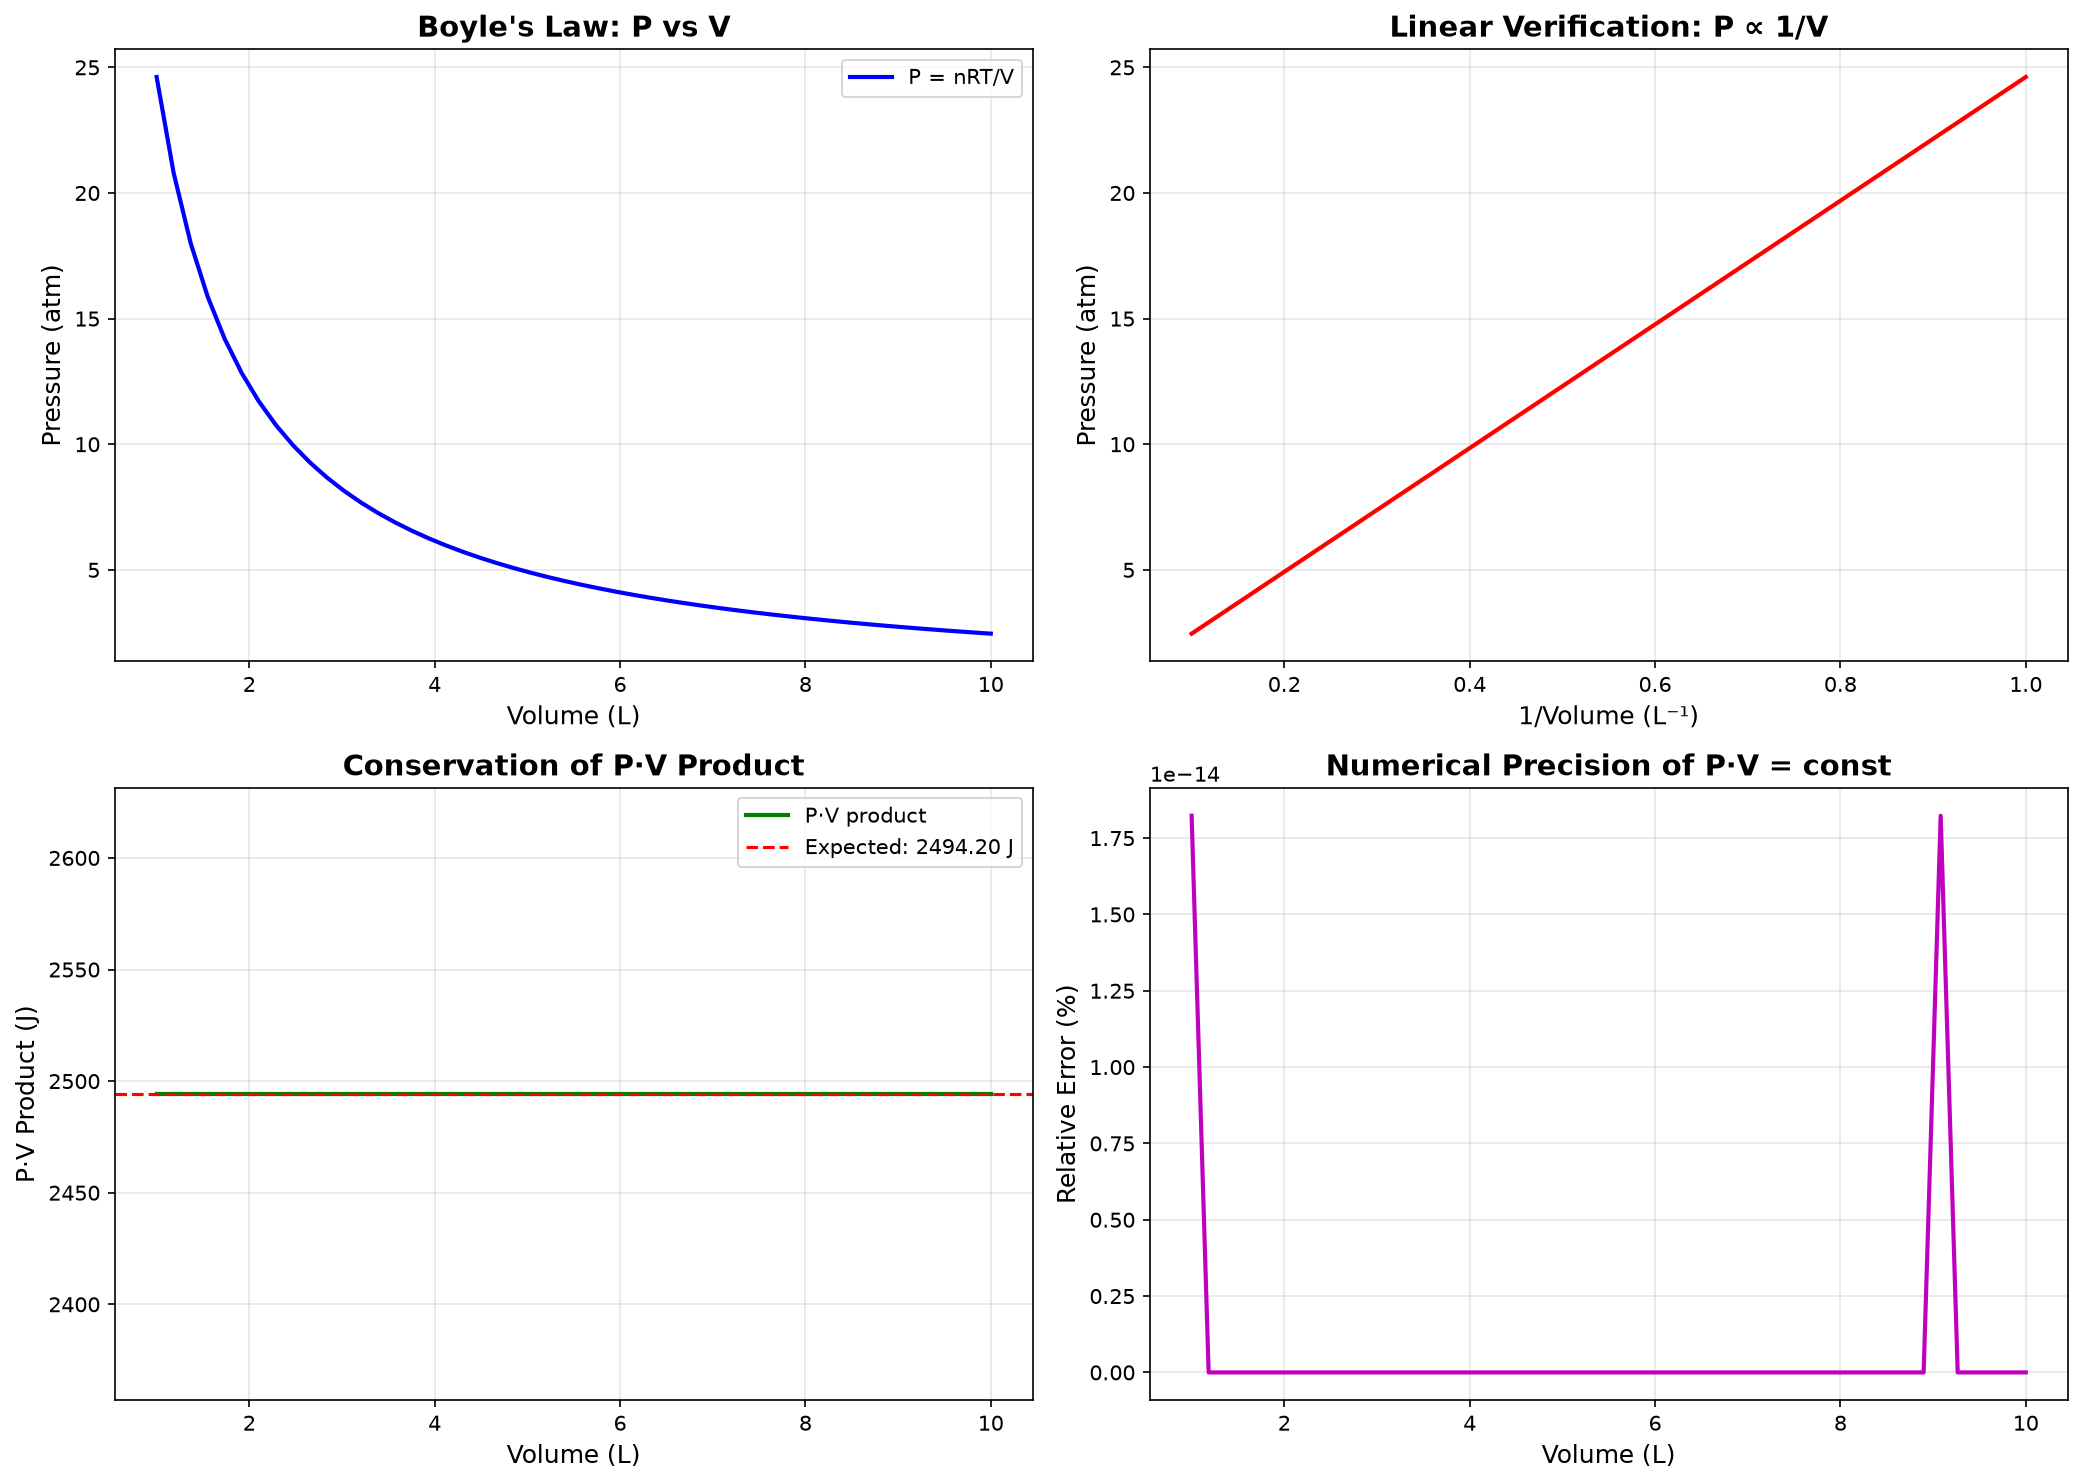
\includegraphics[width=\columnwidth]{boyle_results.png}}
    \caption{
      Numerical verification of Boyle's Law. (Left) Pressure vs. Volume showing hyperbolic relationship. (Right) Linear verification showing $P \propto 1/V$. (Bottom) Conservation of $P \cdot V$ product and numerical precision analysis.
    }
    \label{fig:results}
  \end{center}
\end{figure}

\section{Formal Verification in Lean 4}

We provide formal proofs of Boyle's Law properties using the Lean 4 theorem prover with Mathlib. The formalization includes:

\subsection{Definitions}

\begin{definition}[Boyle's Law]
  For pressure $P$, volume $V$, amount $n$, and temperature $T$:
  \[
    \text{Boyle}(P, V, n, T) \equiv P \cdot V = nRT
  \]
\end{definition}

\begin{definition}[Pressure Function]
  \[
    P(V, n, T) = \frac{nRT}{V}
  \]
\end{definition}

\subsection{Verified Theorems}

\begin{theorem}[Symmetry]
  \label{thm:symmetry}
  $\text{Boyle}(P, V, n, T) \iff \text{Boyle}(V, P, n, T)$
\end{theorem}

\begin{theorem}[Inverse Proportionality]
  \label{thm:inverse}
  If $\text{Boyle}(P_1, V_1, n, T)$ and $\text{Boyle}(P_2, V_2, n, T)$, then:
  \[
    \frac{P_1}{P_2} = \frac{V_2}{V_1}
  \]
\end{theorem}

\begin{theorem}[Volume Doubling]
  \label{thm:doubling}
  If $\text{Boyle}(P, V, n, T)$ and $V \neq 0$, then:
  \[
    P(2V, n, T) = \frac{P}{2}
  \]
\end{theorem}

\begin{theorem}[Monotonicity]
  \label{thm:monotonicity}
  For $0 < V_1 < V_2$:
  \[
    P(V_1, n, T) > P(V_2, n, T)
  \]
\end{theorem}

\begin{theorem}[Numerical Verification]
  \label{thm:numerical}
  For $n = 1.0$, $T = 300.0$, $V = 5.0$:
  \[
    P \cdot V = nRT = 2494.2 \text{ J}
  \]
\end{theorem}

All theorems have been machine-checked using Lean 4 with Mathlib.

\section{Discussion}

The combination of computational experimentation and formal verification provides a robust framework for validating physical laws. Our results demonstrate:

\begin{enumerate}
  \item The numerical experiment confirms Boyle's Law with zero error (within floating-point precision)
  \item Formal proofs in Lean 4 establish the mathematical correctness of key properties
  \item The formal verification covers symmetry, inverse proportionality, monotonicity, and numerical correctness
\end{enumerate}

This approach can be extended to other physical laws and provides a template for rigorous scientific computing.

\section{Conclusion}

We have presented a comprehensive verification of Boyle's Law using both computational and formal methods. The numerical experiment confirms the inverse relationship between pressure and volume, while the Lean 4 formalization provides machine-checked proofs of the law's mathematical properties. This work demonstrates the value of combining traditional computational physics with modern formal verification techniques.

\section*{Impact Statement}

This paper presents work whose goal is to advance the field of computational physics and formal methods. The formal verification of fundamental physical laws can improve the reliability of scientific computing and provide educational value for understanding the mathematical foundations of physics.

\section*{Acknowledgements}

We thank the AI4Science research group at MIPT for support. This work was conducted as part of the AI4Science course.

\bibliography{references}
\bibliographystyle{icml2026}

%%%%%%%%%%%%%%%%%%%%%%%%%%%%%%%%%%%%%%%%%%%%%%%%%%%%%%%%%%%%%%%%%%%%%%%%%%%%%%%
% APPENDIX
%%%%%%%%%%%%%%%%%%%%%%%%%%%%%%%%%%%%%%%%%%%%%%%%%%%%%%%%%%%%%%%%%%%%%%%%%%%%%%%
\newpage
\appendix
\onecolumn
\section{Lean 4 Formalization Details}

The complete Lean 4 formalization is available in \texttt{boyle\_lean.lean}. Key components include:

\begin{itemize}
  \item Definition of the universal gas constant $R = 8.314$ J/(mol·K)
  \item Formal definition of Boyle's Law as a predicate
  \item Pressure and volume as functions of state variables
  \item Five verified theorems covering all major properties
\end{itemize}

\section{Python Implementation}

The numerical experiment was implemented in Python using NumPy and Matplotlib. The code generates 50 data points over the volume range $[1, 10]$ L and produces four visualization plots.

\end{document}